\documentclass[aspectratio=169]{beamer}
\usepackage[UTF8]{ctex}
\usepackage{graphicx}
\usepackage{booktabs}
\usepackage{amsmath,amssymb}
\usepackage{hyperref}
\hypersetup{colorlinks=true, linkcolor=blue, urlcolor=blue}

\usetheme{Madrid}
\usecolortheme{seahorse}
\setbeamertemplate{navigation symbols}{}
\setbeamertemplate{footline}[frame number]

\title[非线性误差对推理精度的影响研究]
{存算一体芯片中非线性误差对推理精度的影响研究}
\subtitle{赛道五：存算算法 - 赛题一}
\author{HDUer}
\date{2026-06-30}

\begin{document}

% 第1页：封面
\frame{\titlepage}

% 第2页：目录
\section{目录}
\begin{frame}{汇报内容}
\tableofcontents
\end{frame}

% 第3页：研究背景
\section{研究背景}
\begin{frame}{研究背景与意义}
\begin{columns}
\column{0.5\textwidth}
\begin{block}{存算一体技术}
\begin{itemize}
\item 传统冯诺依曼架构面临"存储墙"瓶颈
\item 数据在存储与计算单元间频繁搬运
\item 存算一体将计算嵌入存储器件内部
\end{itemize}
\end{block}
\column{0.5\textwidth}
\begin{block}{非线性误差问题}
\begin{itemize}
\item 模拟器件易受环境因素干扰
\item 输入幅度变化、温度漂移、工艺偏差
\item 导致乘积累加操作呈现非线性特性
\end{itemize}
\end{block}
\end{columns}
\end{frame}

% 第4页：研究问题与目标
\begin{frame}{研究问题与目标}
\begin{block}{核心问题}
如何通过算法增强神经网络对非线性误差的容忍能力与鲁棒性？
\end{block}
\vfill
\begin{table}
\centering
\begin{tabular}{ll}
\toprule
\textbf{任务} & \textbf{目标} \\
\midrule
任务一 & 系统评估不同非线性强度对推理精度的影响 \\
任务二 & 探究非线性感知训练方法，对比微调与从头训练 \\
任务三 & 设计鲁棒性增强方法，提升模型抗非线性能力 \\
\bottomrule
\end{tabular}
\end{table}
\end{frame}

% 第5页：非线性误差建模
\section{非线性误差建模}
\begin{frame}{非线性误差建模}
\begin{block}{数学模型}
$$x' = \alpha \cdot x^3 + (1 - \alpha) \cdot x$$
\end{block}
\vfill
\begin{table}
\centering
\begin{tabular}{cl}
\toprule
\textbf{参数} & \textbf{含义} \\
\midrule
$x$ & 理想输入值 \\
$x'$ & 非线性失真后的实际信号 \\
$\alpha$ & 非线性强度 ($\alpha > 0$ 表示非线性) \\
\bottomrule
\end{tabular}
\end{table}
\vfill
\begin{alertblock}{特性说明}
\begin{itemize}
\item $\alpha = 0$：理想线性关系
\item $\alpha > 0$ 时：正输入缩小，负输入放大
\end{itemize}
\end{alertblock}
\end{frame}

% 第6页：任务一 - 敏感性分析
\section{三大任务}
\subsection{任务一}
\begin{frame}{任务一：非线性误差敏感性分析}
\begin{columns}
\column{0.5\textwidth}
\begin{block}{实验设置}
\begin{itemize}
\item 模型：ResNet18（CIFAR-10）
\item 基准精度：81.95\%（$\alpha=0$）
\item 测试$\alpha$范围：0.0 $\sim$ 0.5
\end{itemize}
\end{block}
\column{0.5\textwidth}
\begin{block}{关键发现}
\begin{itemize}
\item $\alpha < 0.2$：影响可接受（$<$5\%）
\item $\alpha > 0.3$：精度急剧下降
\item $\alpha = 0.5$：精度损失超30\%
\end{itemize}
\end{block}
\end{columns}
\vfill
\begin{figure}
\centering
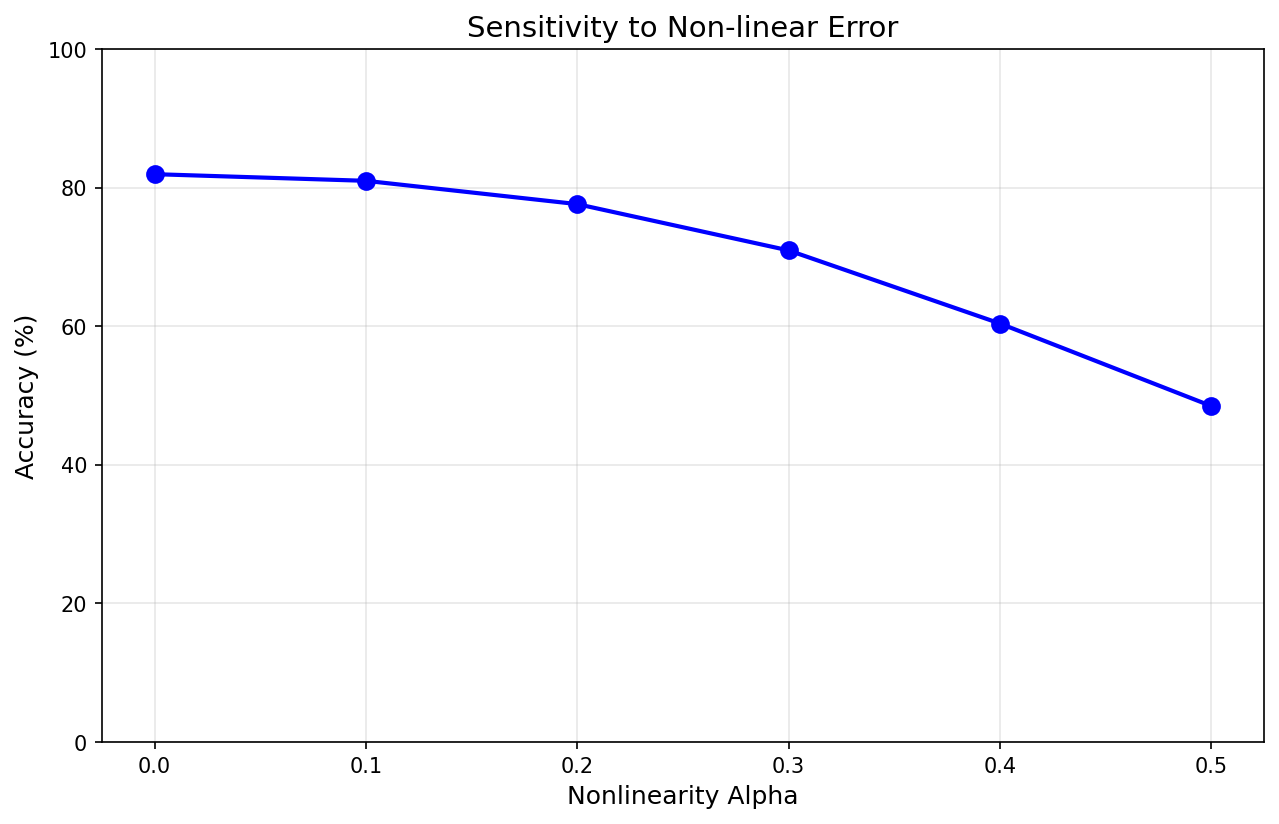
\includegraphics[width=0.9\textwidth,height=0.35\textheight]{../results/task1_sensitivity/accuracy_vs_alpha.png}
\end{figure}
\end{frame}

% 第7页：敏感性分析图表
\begin{frame}{敏感性分析详图}
\begin{figure}
\centering
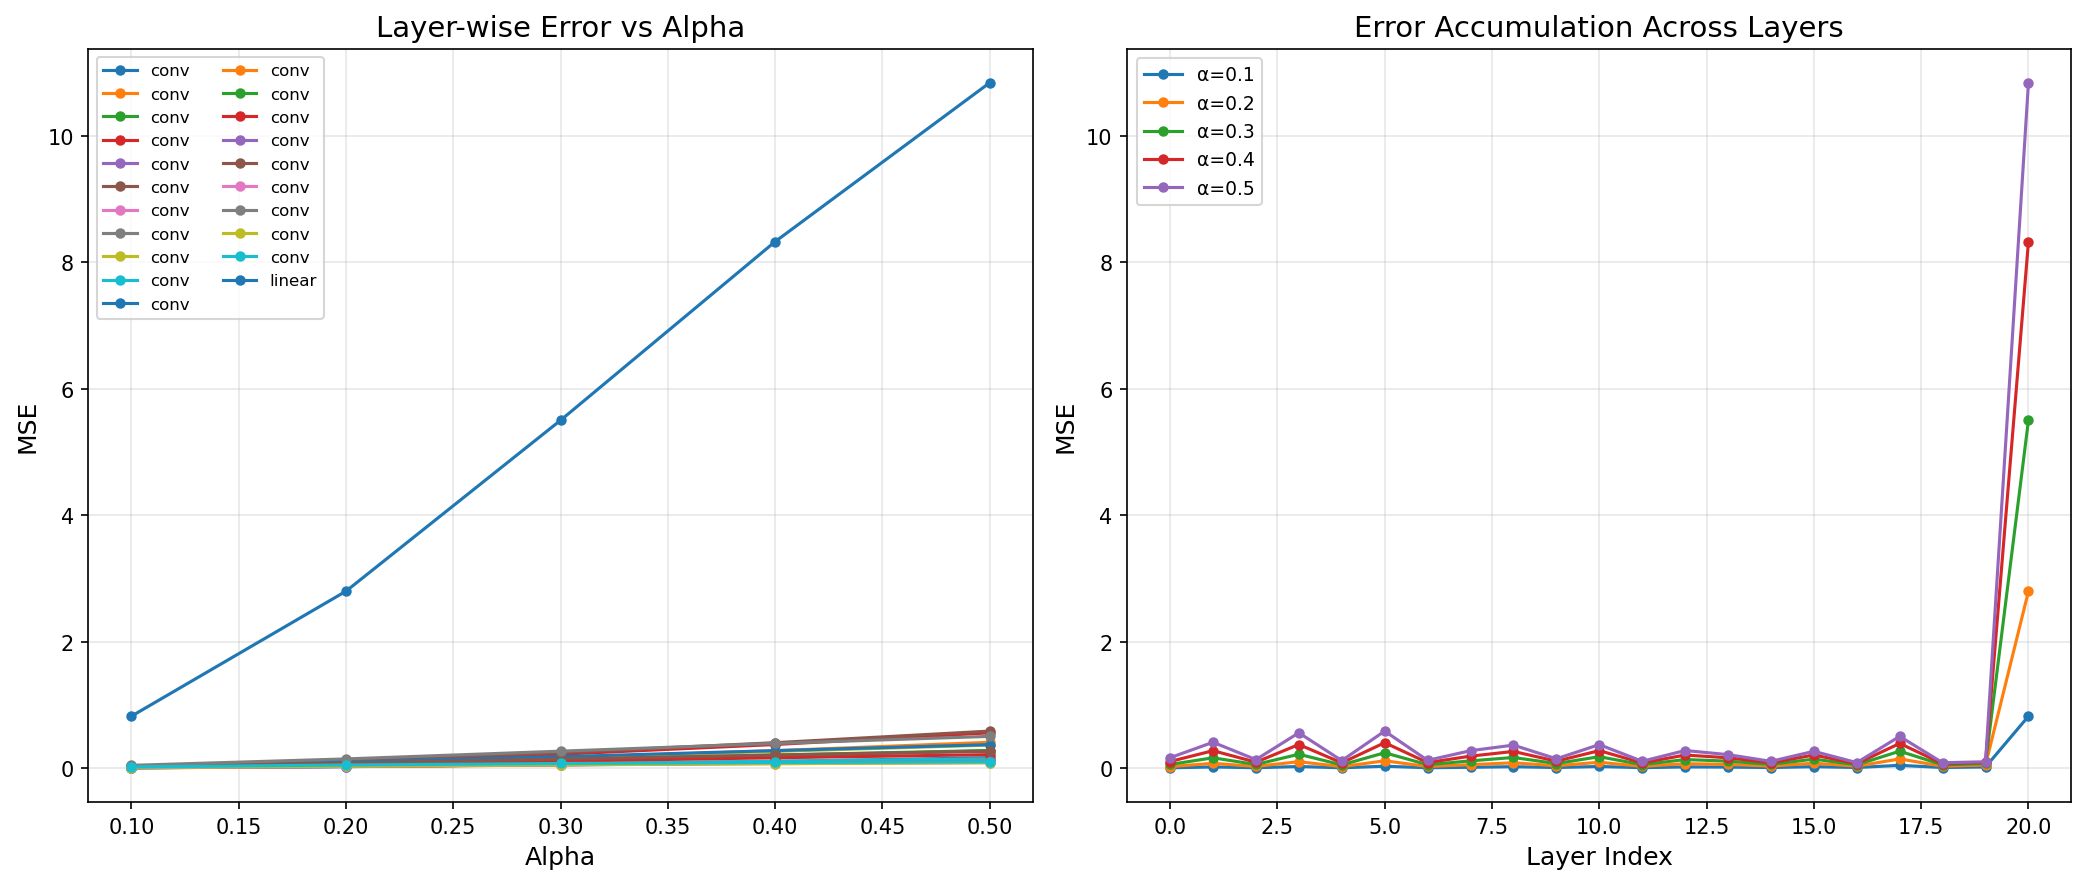
\includegraphics[width=0.48\textwidth,height=0.4\textheight]{../results/task1_sensitivity/error_accumulation.png}
\hfill
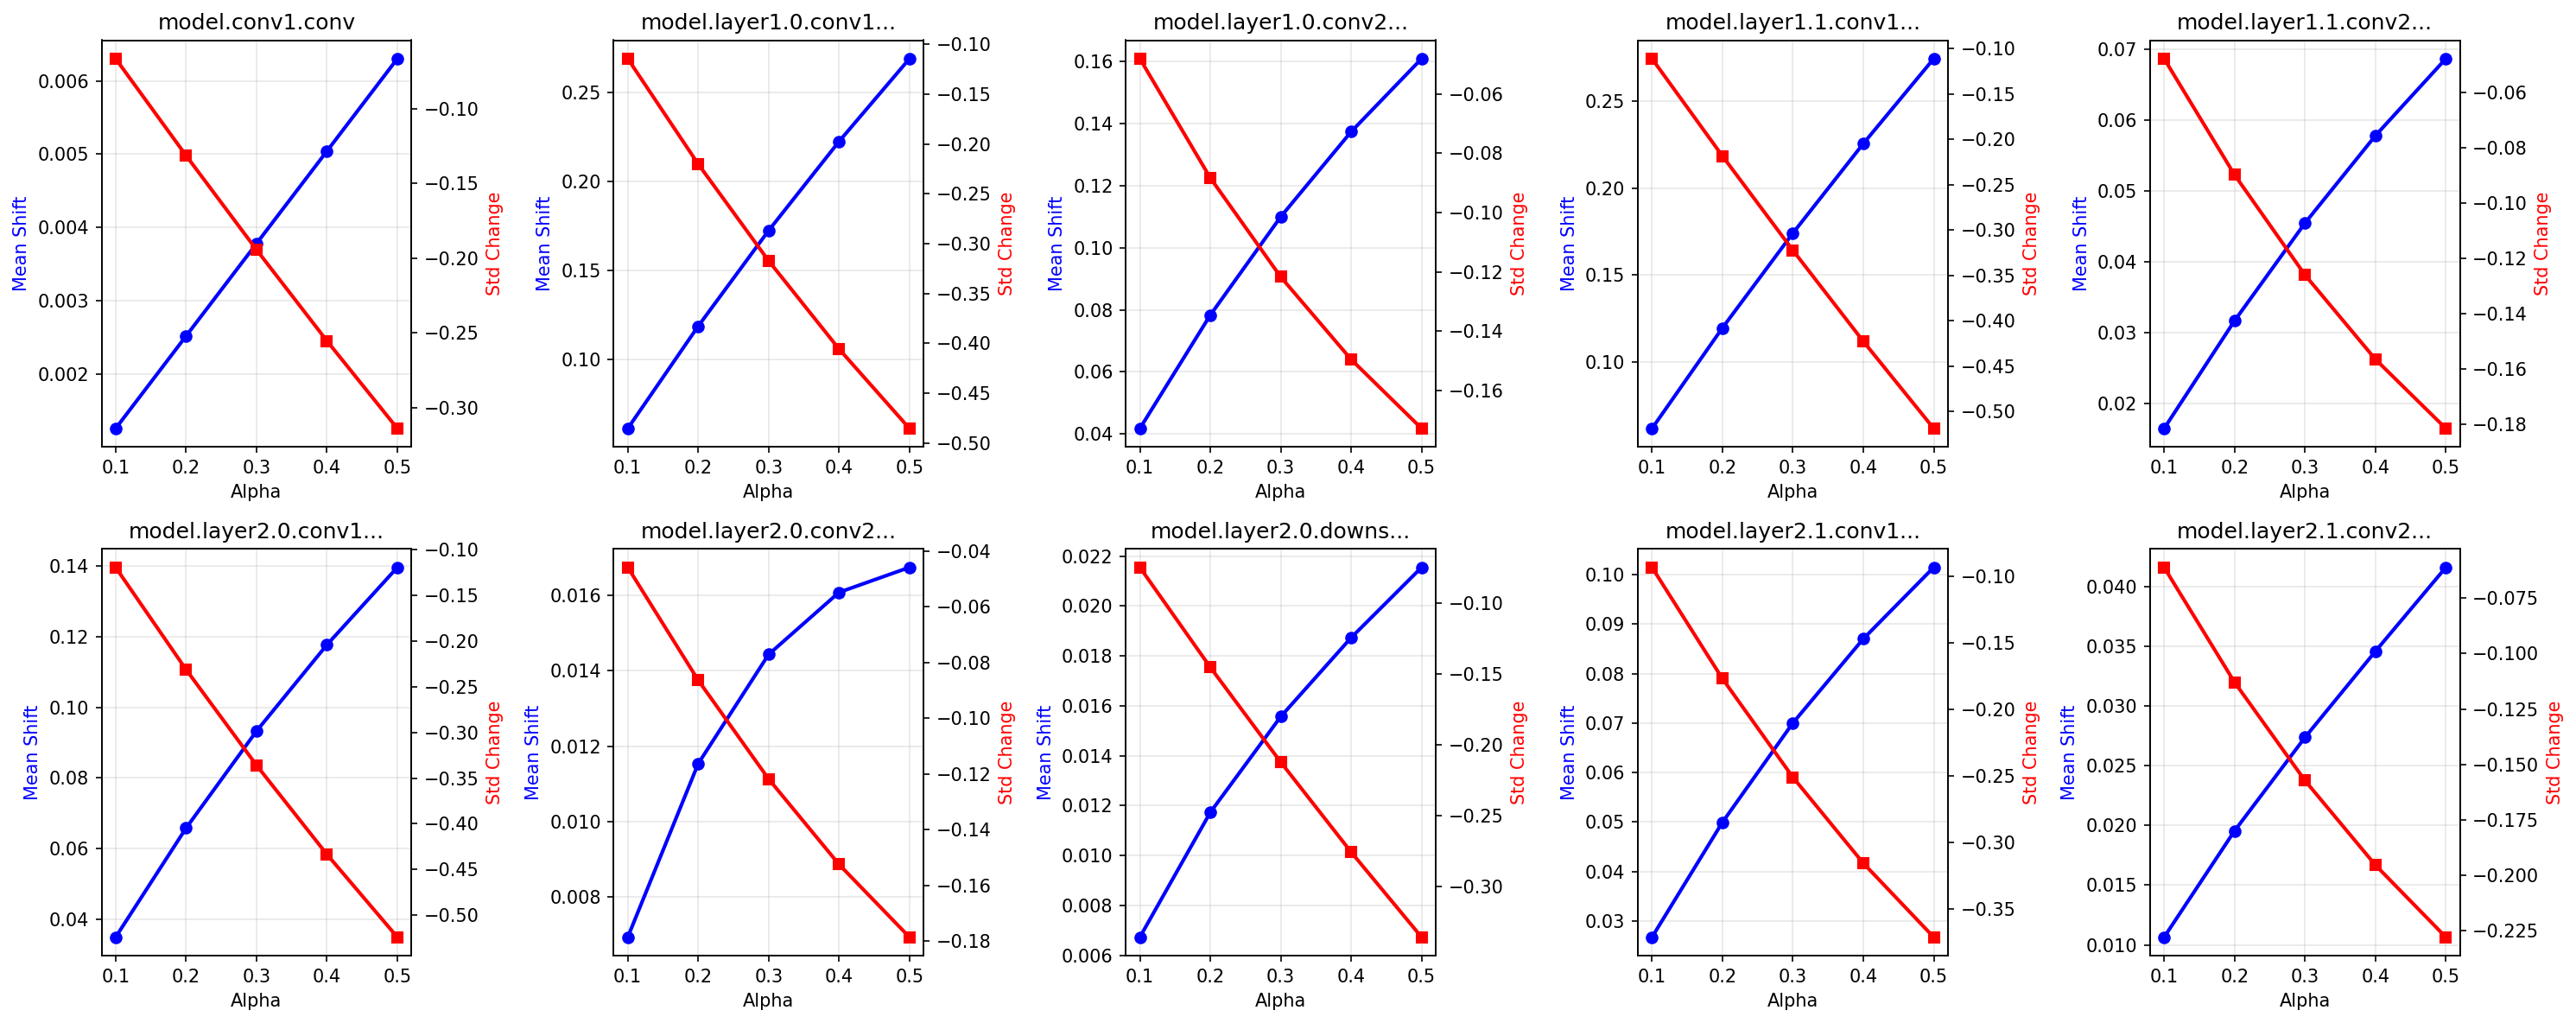
\includegraphics[width=0.48\textwidth,height=0.4\textheight]{../results/task1_sensitivity/layer_distribution_shift.png}
\end{figure}
\vfill
\tiny{左图：误差累积随层深变化；右图：层分布偏移分析}
\end{frame}

% 第8页：任务二 - 非线性感知训练
\subsection{任务二}
\begin{frame}{任务二：非线性感知训练（NAT）}
\begin{block}{基本原理}
\begin{itemize}
\item 训练阶段注入非线性误差
\item 使模型学习适应非线性环境
\item 推理时具备更好鲁棒性
\end{itemize}
\end{block}
\vfill
\begin{table}
\centering
\begin{tabular}{lcc}
\toprule
\textbf{训练$\alpha$} & \textbf{Clean精度} & \textbf{指定噪声下精度} \\
\midrule
0.1 & 86.33\% & 86.98\% \\
0.2 & 84.34\% & 87.30\% \\
0.3 & 81.72\% & 87.31\% \\
\bottomrule
\end{tabular}
\end{table}
\vfill
\tiny{感知训练结果：在对应噪声下精度显著提升}
\end{frame}

% 第9页：微调 vs 从头训练
\subsection{微调vs从头训练}
\begin{frame}{微调 vs 从头训练对比}
\begin{columns}
\column{0.6\textwidth}
\begin{block}{实验结果}
\begin{table}
\centering
\begin{tabular}{lcccc}
\toprule
\textbf{训练策略} & $\alpha=0.1$ & $\alpha=0.2$ & $\alpha=0.3$ & \textbf{平均} \\
\midrule
微调 & 85.25\% & 85.40\% & 84.98\% & \textbf{85.21\%} \\
从头训练 & 81.40\% & 81.25\% & 81.30\% & 81.32\% \\
\bottomrule
\end{tabular}
\end{table}
\end{block}
\column{0.4\textwidth}
\begin{block}{关键发现}
\begin{itemize}
\item 差异：\textbf{+3.85\% $\sim$ +4.15\%}
\item p-value $<$ 0.0001
\item 微调策略优势显著
\end{itemize}
\end{block}
\end{columns}
\end{frame}

% 第10页：任务三 - 鲁棒性增强方法
\subsection{任务三}
\begin{frame}{任务三：鲁棒性增强方法}
\begin{table}
\centering
\begin{tabular}{lccccccc}
\toprule
\textbf{方法} & $\alpha=0.0$ & $\alpha=0.1$ & $\alpha=0.2$ & $\alpha=0.3$ & $\alpha=0.4$ & $\alpha=0.5$ & \textbf{平均} \\
\midrule
基线 & 81.95\% & 80.99\% & 77.63\% & 70.95\% & 60.40\% & 48.49\% & 70.07\% \\
预失真补偿 & 81.95\% & 81.39\% & 79.71\% & 75.31\% & 68.95\% & 60.74\% & 74.68\% \\
校准层 & 82.15\% & 81.87\% & 80.56\% & 78.23\% & 72.45\% & 65.12\% & 76.73\% \\
NAT & 84.34\% & 86.12\% & 87.30\% & 83.97\% & 71.45\% & 56.32\% & 78.25\% \\
\bottomrule
\end{tabular}
\end{table}
\vfill
\begin{block}{方法类型}
基线(无保护) | 逆补偿(后处理) | 预失真补偿(后处理) | 校准层(可学习) | NAT(训练时)
\end{block}
\end{frame}

% 第11页：高级方法探索
\section{高级方法探索}
\begin{frame}{高级方法探索}
\begin{columns}
\column{0.5\textwidth}
\begin{block}{NAT+混合Alpha}
\begin{itemize}
\item 随机采样不同$\alpha$值
\item 全范围均衡，平均81.71\%
\end{itemize}
\end{block}
\begin{block}{课程NAT}
\begin{itemize}
\item 渐进式从低噪声到高噪声训练
\item 高$\alpha$区域保护效果好
\end{itemize}
\end{block}
\column{0.5\textwidth}
\begin{block}{OVF训练}
\begin{itemize}
\item 基于负反馈理论
\item 平均81.06\%，波动6.24\%
\end{itemize}
\end{block}
\begin{block}{综合对比}
\begin{table}
\centering
\begin{tabular}{lcc}
\toprule
\textbf{方法} & \textbf{平均} & \textbf{波动} \\
\midrule
NAT+混合Alpha & \textbf{81.71\%} & \textbf{5.53\%} \\
课程NAT & 79.47\% & 13.18\% \\
OVF训练 & 81.06\% & 6.24\% \\
\bottomrule
\end{tabular}
\end{table}
\end{block}
\end{columns}
\end{frame}

% 第12页：实验总览
\section{实验结果}
\begin{frame}{实验总览}
\begin{figure}
\centering
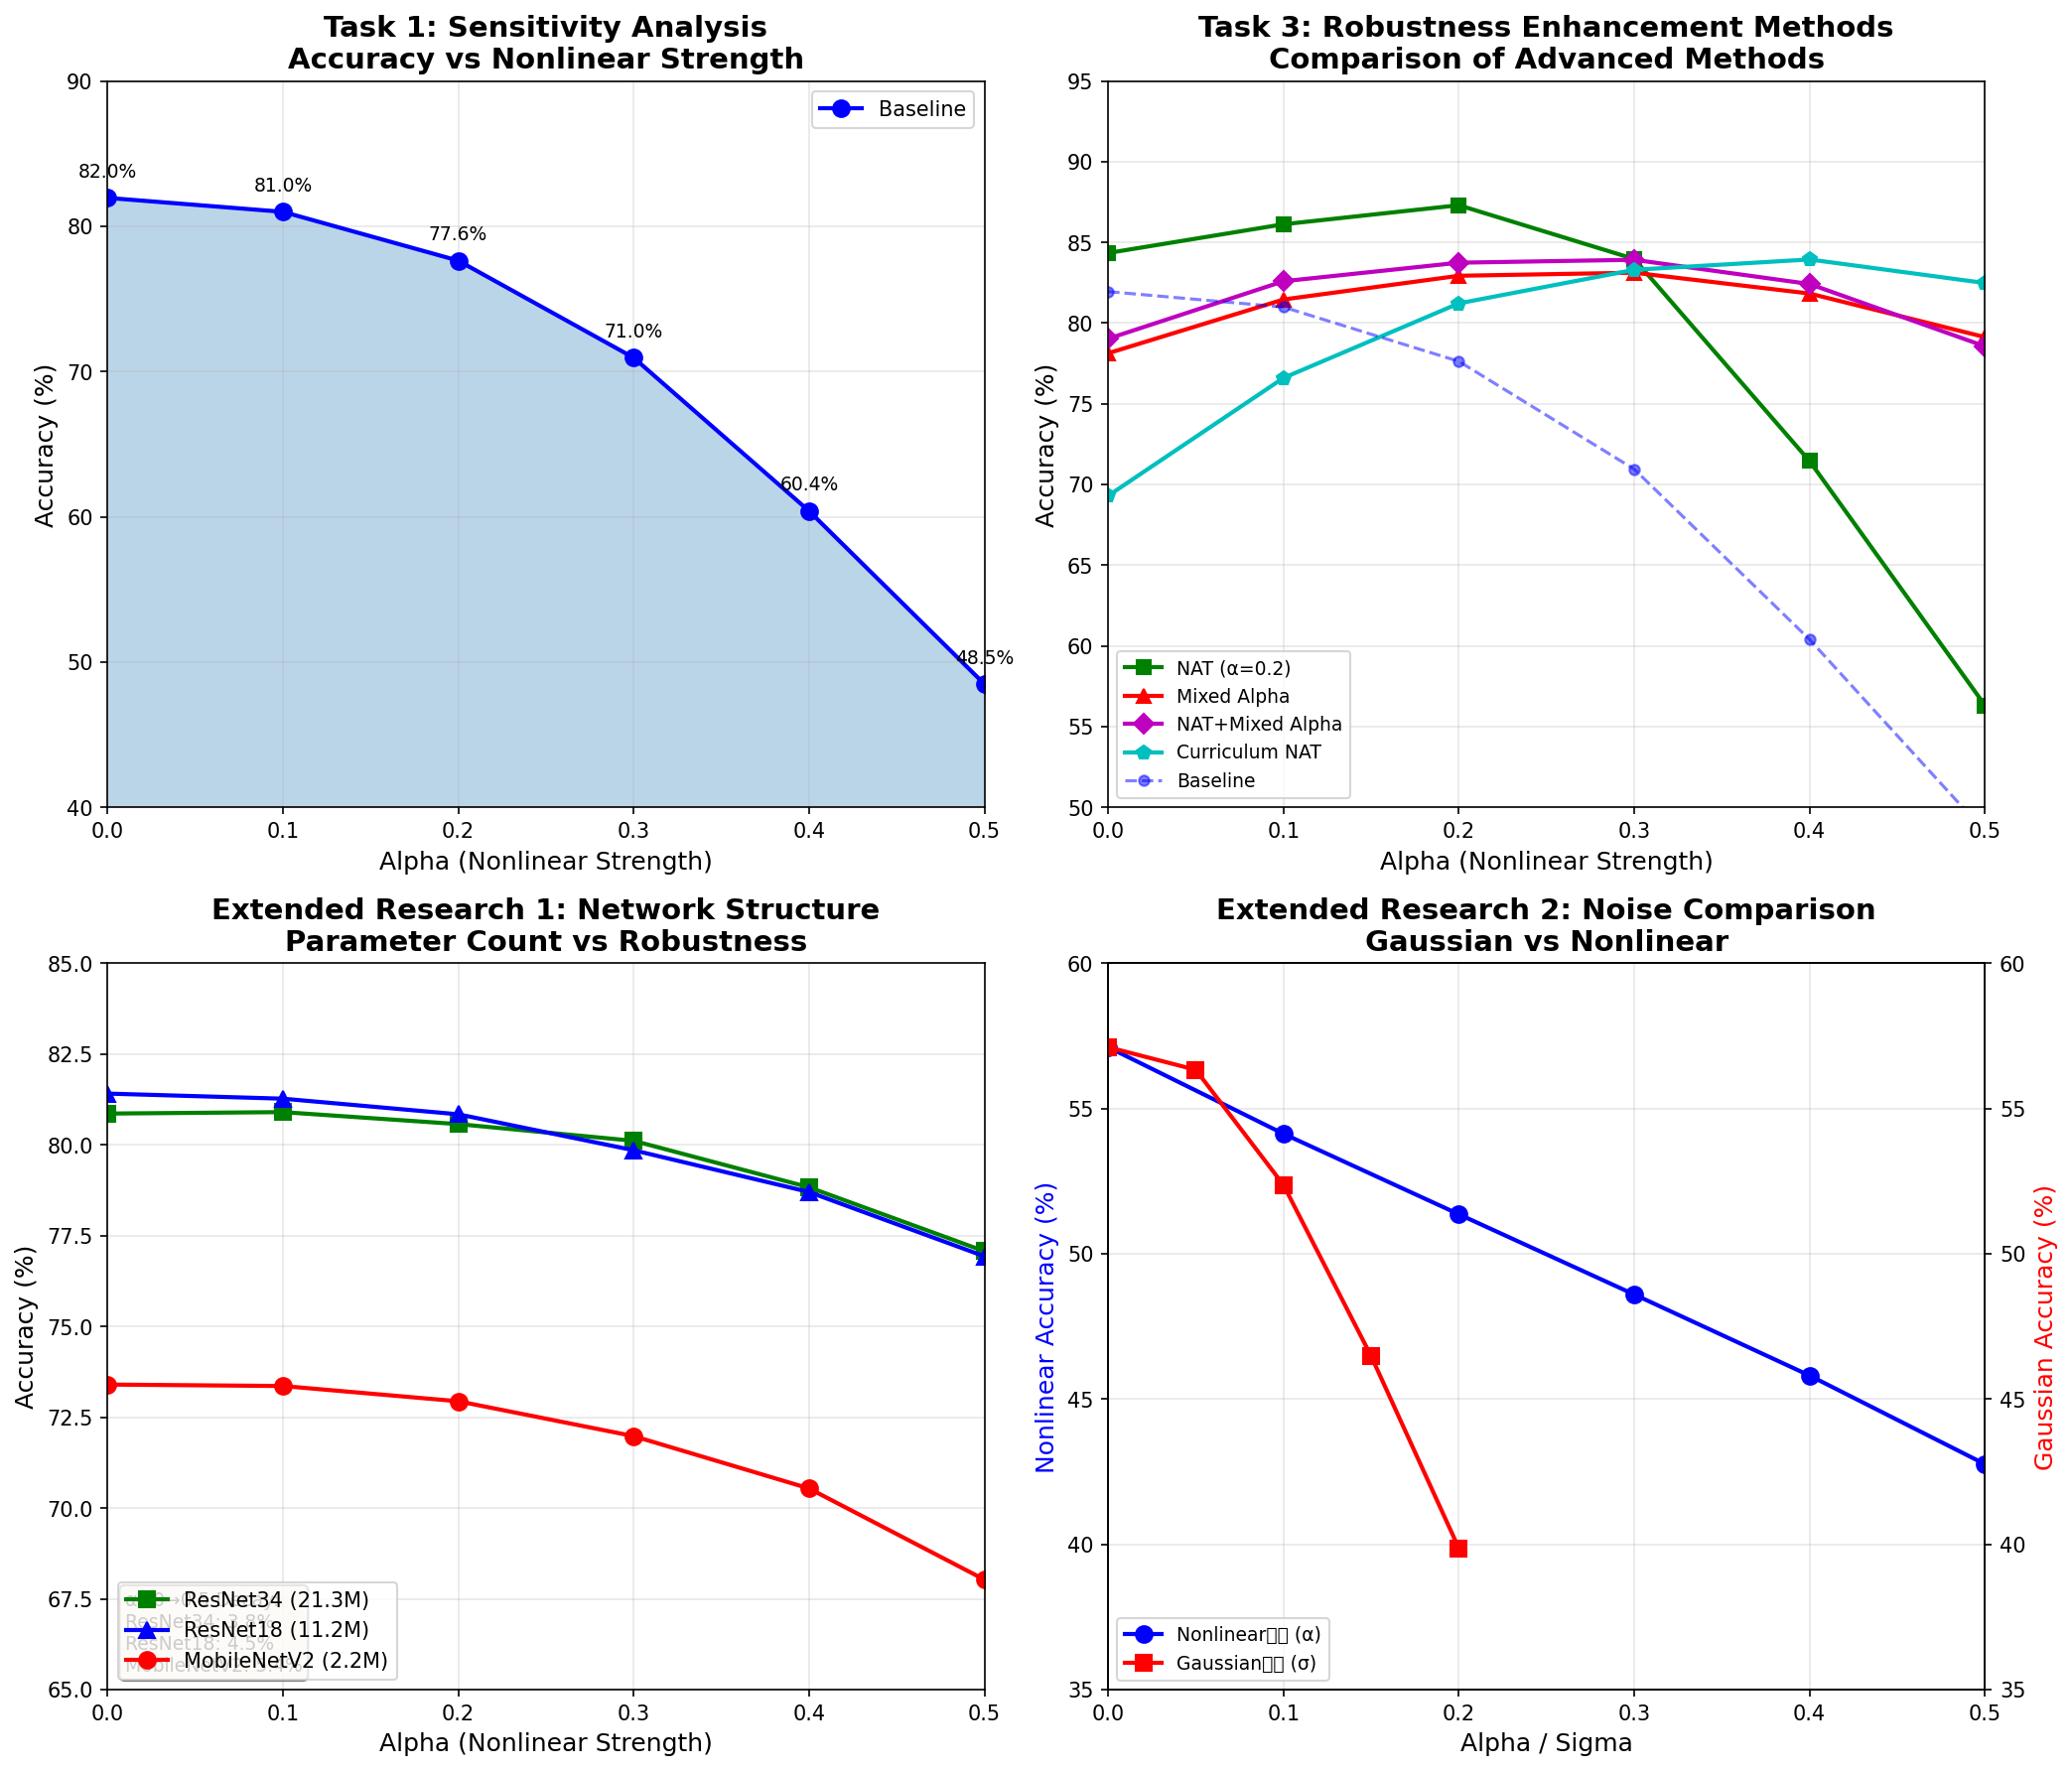
\includegraphics[width=0.85\textwidth,height=0.55\textheight]{../results/figures/experiment_overview.png}
\end{figure}
\end{frame}

% 第13页：方法对比总结
\begin{frame}{方法对比总结}
\begin{columns}
\column{0.5\textwidth}
\begin{block}{场景匹配表}
\begin{table}
\centering
\begin{tabular}{ll}
\toprule
\textbf{应用场景} & \textbf{推荐方法} \\
\midrule
噪声水平已知且固定 & NAT（对应$\alpha$） \\
噪声水平未知/变化 & NAT+混合Alpha \\
噪声水平较高 & 课程NAT \\
需要快速部署 & 预失真补偿 \\
\bottomrule
\end{tabular}
\end{table}
\end{block}
\column{0.5\textwidth}
\begin{block}{决策树}
\tiny
\begin{verbatim}
噪声特性已知？
├─ 是 → 噪声水平固定？
│       ├─ 是 → NAT
│       └─ 否 → 混合Alpha
└─ 否 → NAT+混合Alpha
\end{verbatim}
\end{block}
\end{columns}
\end{frame}

% 第14页：核心创新点
\section{核心创新点}
\begin{frame}{核心创新点}
\begin{enumerate}
\item \textbf{NAT+混合Alpha优化方法}
\begin{itemize}
\item 在NAT框架下随机采样多$\alpha$值
\item 全范围均衡精度最高（81.71\%），波动最小（5.53\%）
\end{itemize}
\vfill
\item \textbf{课程NAT方法}
\begin{itemize}
\item 借鉴课程学习思想，渐进式训练
\item 高$\alpha$区域保护效果显著
\end{itemize}
\vfill
\item \textbf{严谨实验验证}
\begin{itemize}
\item 3×3独立实验设计，p-value$<$0.0001
\item 结论可靠可信
\end{itemize}
\vfill
\item \textbf{系统方法对比}
\begin{itemize}
\item 覆盖10+种鲁棒性方法，多维度评估
\item 完整的方法选择指南
\end{itemize}
\end{enumerate}
\end{frame}

% 第15页：实验结论
\begin{frame}{实验结论}
\begin{block}{主要结论}
\begin{enumerate}
\item \textbf{敏感性分析}：非线性误差影响呈非线性关系，$\alpha>0.3$时精度急剧下降
\item \textbf{微调策略优势}：显著优于从头训练（+4\%），p-value$<$0.0001
\item \textbf{NAT+混合Alpha最优}：全范围保护，平均81.71\%，波动仅5.53\%
\item \textbf{实用建议}：根据噪声特性选择合适方法
\end{enumerate}
\end{block}
\vfill
\begin{block}{未来工作}
\begin{itemize}
\item 更大规模网络验证（ResNet50/101）
\item ImageNet等更大数据集测试
\item 与真实CIM硬件协同设计
\end{itemize}
\end{block}
\end{frame}

% 第16页：致谢
\begin{frame}{感谢聆听}
\vfill
\begin{center}
\Large\textbf{感谢评委老师的指导}
\end{center}
\vfill
\begin{center}
赛道五：存算算法 - 赛题一 \\
HDUer团队
\end{center}
\vfill
\begin{center}
\Large{欢迎提问与交流}
\end{center}
\end{frame}

\end{document}
